
\chapter{Návrh grafického programovacieho jazyka}
\label{kap:navrh-gpj}

V kapitole opisujeme priebeh vzniku grafického programovacieho jazyka použitého v našej aplikácii. Rôzne verzie (kapitola \ref{sec:system-verzii}) vyžadujú sprístupnenie rôznych komponentov. Hlavným predmetom tvorby GPJ pomocou knižnice Blockly je definícia blokov a im prislúchajúcich generátorov (kapitola \ref{kap:GrafickyProgramovaciJayzk}).


%%%%%
% %%% 	Verzia Otto 2020 Robotická liga
%%%%%
\section{Verzia Otto 2020 Robotická liga}
V tejto verzii je možné tvoriť choreografie pre robota Otto ako postupnosť trojíc celých čísel (kapitola \ref{sub:otto} a \ref{sub:verzia-otto-2020-rl}). Formát a význam jednotlivých čísel je uvedený na web stránke Denného tábora digitálnych technológií prezentujúcej robota Otto \cite{ottoChoreographies}. Základom sú trojice pre ovládanie motorov, k dispozícii sú ale i ďalšie, umožňujúce ovládanie prehrávania melódie či zvukových efektov (tabuľka \ref{tab:otto-choreograpies-tab}). Celá choreografia, sériovou linkou prenášaná do mikropočítača, má formát \uv{$@\;x_1\;y_1\;z_1\;x_2\;y_2\;z_2\;...\;x_n\;y_n\;z_n\;0\;0\;0 $}, kde vždy trojica (príkaz) pozostáva z hodnôt ($x_i, y_i, z_i$).

\begin{table}\footnotesize
\centering
\newcolumntype{P}[1]{>{\centering\arraybackslash}p{#1}}
\begin{tabular}{ |P{1cm}P{0.6cm}P{1cm}|p{11.2cm}| }
	\hline
	\multicolumn{3}{|c|}{\textbf{formát príkazu}}&\textbf{význam} \\
	\hline
	$X$ & $Y$   & $Z$ & počkaj $X$ ms, pohni motorom $Y$ do polohy $Z$; $Y\in [1;6]; Z\in [0,180]$  \\
	1 & 8   & $X$ & nastav celkový čas prehrávania choreografie na $X$ sekúnd \\
	1 & 9   & $X$ & pokračuj príkazom na riadku $X$ \\
	1 & 10 & $X$ & nastav spomalenie pohybu, 0= bez spomalenia \\
	1 & 11 & $X$ & začni hrať melódiu číslo $X$, 0 = vypnúť zvuk \\
	1 & 12 & $X$ & zahraj zvukový efekt číslo $X$ \\
	1 & 13 & 0 & zastav prehrávanie melódie \\
	1 & 14 & $X$ & začni hrať pesničku číslo $X$ \\
	1 & 15 & 0 & vypni / zapni reproduktor \\
	\hline
 \end{tabular}
\caption{\label{tab:otto-choreograpies-tab}Prípustné hodnoty v zápise choreografie robota Otto pomocou trojíc čísel}
\end{table}\normalsize

Na základe tabuľky \ref{tab:otto-choreograpies-tab} vytvárame v GPJ bloky pre jednotlivé funkcie (trojice). Cieľom je zachovať rozsah funkcionalít, no ponúknuť atraktívnejší a pohodlnejší prístup k tvorbe choreografie tohoto formátu. Jednotlivé bloky sú interpretované jednoducho ako prislúchajúca trojica celých čísel.

Príklad choreografie vytvorenej pomocou vzniknutých blokov možno vidieť na obrázku \ref{obr:otto-rl-blockly-general-example}. Bloky vyžadujúce zadanie parametra majú v tele dostupné pole, kde je možné príslušnú hodnotu určiť. Na obrázku \ref{obr:otto-rl-blockly-general-example} ide napríklad o bloky pre nastavenie spomalenia alebo blok pre spustenie prehrávania melódie. V prípade bloku pre riadenie pohybu motora zavádzame možnosť výberu konkrétneho motora z ponuky, namiesto zadania jeho čísla. Zavádzame tiež blok \uv{Program}, do ktorého tela sú vkladané ostatné bloky --- prvky choreografie. Blok \uv{Program} je v tejto verzii statickým prvkom pracovnej plochy editora GPJ, používateľ ho nemôže odstrániť ani duplikovať. Slúži na ohraničenie blokov, ktoré tvoria choreografiu. Bloky umiestnené v editore mimo telo tohto bloku nie sú brané do úvahy pri generovaní kódu. Výsledný program po preložení blokov môžete vidieť v ukážke \ref{OttoRlGeneralExampleCode}.

\begin{figure}
\centerline{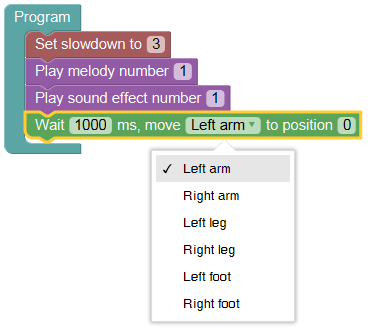
\includegraphics[width=0.6\textwidth]{images/otto-rl-blockly-general}}
\caption[Ukážka kódu v GPJ pre verziu Otto RL 2020]{Ukážka kódu v GPJ pre verziu Otto RL 2020}
\label{obr:otto-rl-blockly-general-example}
\end{figure}

\lstset{language=C,caption={Kód generovaný z blokov na obrázku \ref{obr:otto-rl-blockly-general-example}},label=OttoRlGeneralExampleCode}
\begin{lstlisting}[frame=single]
@1 10 3
1 11 1
1 12 1
1000 5 0
0 0 0
\end{lstlisting}


%%%%%
% %%% 	Verzia Otto 2021 Procedural
%%%%%
\section{Verzia Otto 2021 Procedural}
V tejto verzii sprístupňujeme v GPJ prvky pre tvorbu riadiaceho programu v jazyku Arduino (C++). Použité bloky sú členené do kategórií. Každá kategória zodpovedá \uv{tematickému} celku, prípadne logickému modulu verzie. Podľa zavedených kategórií sú bloky zobrazené v ponuke v používateľskom rozhraní. Nižšie uvádzame ich zoznam.

\begin{itemize}[topsep=8pt,itemsep=0.1pt,partopsep=4pt, parsep=4pt]
\item Matematická logika (podmienka if, logické operácie, pravdivostné hodnoty)
\item Cykly (cyklus for, while a blok pre príkazy \textit{break} a \textit{continue})
\item Matematika (číselné konštanty, aritmetické operácie, náhodné čísla)
\item Premenné (možnosť tvorby premenných rôznych typov)
\item Funkcie (možnosť tvorby procedúr a funkcií)
\item Zvuk (ovládanie zvukových efektov a mp3 prehrávača)
\item Pohyb (ovládanie servomotorov)
\item Senzory (prístup k funkciám dotykových tlačidiel a ultrazvukovému senzoru)
\item Sériová komunikácia (prijímanie a odosielanie správ cez pripojený USB kábel)
\item Sériová komunikácia cez Bluetooth
\item Práca s časom
\item Špecifické funkcie robota Otto
\end{itemize}

Knižnica Blockly poskytuje základné, všeobecné bloky \uv{od výroby}. K dispozícii sú bloky pre \textit{vetvenie programu podmienkou if}, bloky pre \textit{cykly}, bloky pre \textit{logické a číselné konštanty} a manipuláciu s nimi (základná aritmetika a logické operácie), bloky pre \textit{manipuláciu s textom}, \textit{tvorbu zoznamov}, \textit{reprezentáciu a miešanie farieb}, \textit{tvorbu premenných} a \textit{definíciu procedúr a funkcií}. Súčasťou sú generátory pre jazyky JavaScript, Python, Dart, Lua a PHP, z ktorých možno vychádzať. Niektoré z týchto blokov použijeme i v našej aplikácii, najmä definíciu ich vizuálnej podoby. Syntax jazyka C však vyžaduje redefiníciu generátorov viacerých prebraných blokov. K prebraným častiam patria bloky pre logické operácie, cykly, definície procedúr a funkcií, matematické operácie a premenné. Dôležitými pre našu aplikáciu sú však najmä novovzniknuté bloky, umožňujúce obsluhu špecifických funkcií robota. V knižnici dotvárame bloky umožňujúce pohyb, čítanie hodnôt meraných senzormi, sériovú komunikáciu či komunikáciu rozhraním Bluetooth. 

Komplexitou funkcie poskytovanej blokom je možné nastaviť úroveň abstrakcie. Jednoduchým príkladom je blok \uv{čakanie na stlačenie tlačidla} (obrázok \ref{obr:wait-till-couch}). Možno ho ľahko vyskladať z blokov \textit{cyklu while}, \textit{negácie} a bloku pre \textit{načítanie stavu tlačidla} (na obrázku vľavo), no najmä pre nižšie vekové kategórie je vhodnejšia alternatíva vyššej abstraktnej úrovne (na obrázku vpravo). Iným príkladom je blok pre načítanie gesta pomocou ultrazvukového senzora, ktorý reprezentuje v pozadí pomerne zložitú implementáciu časti riadiaceho programu, zabezpečujúcu komunikáciu s hardvérom a elimináciu chyby opakovaným meraním. V rámci jednotlivých kategórií je preto našou snahou poskytnúť bloky rôzneho charakteru, s rôznou komplexitou a úrovňou abstrakcie.

\begin{figure}
\centerline{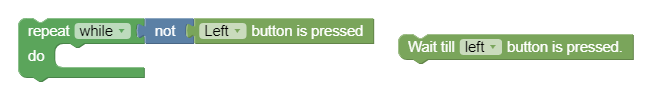
\includegraphics[width=1\textwidth]{images/wait-till-couch}}
\caption[Blockly --- abstrakcia bloku \uv{čakaj na stlačenie tlačidla}]{Blockly --- abstrakcia bloku \uv{čakaj na stlačenie tlačidla}}
\label{obr:wait-till-couch}
\end{figure}

I v tejto verzii zavádzame v editore GPJ fixný, statický blok \uv{Program}, ktorý reprezentuje časť \textit{loop} riadiaceho programu v Arduino a všetok kód je tvorený pridávaním blokov do jeho tela. Bloky bez pripojenia (priameho a zároveň nepriameho) k tomuto bloku nie sú pri vyhodnocovaní (generovaní kódu) brané do úvahy. Výnimku majú len bloky umiestnené v tele blokov definujúcich funkcie a procedúry. Príklad možno vidieť na obrázku \ref{obr:disabled-orphan-block}. Je tu zobrazený obsah pracovnej plochy editora GPJ. Blok vľavo bude pri generovaní C++ kódu vyhodnotený, ide o hlavný blok \uv{Program}, ktorého obsah tvorí časť \textit{loop} riadiaceho programu Arduino. Blok v strede, definujúci procedúru \uv{do something}, bude tiež vyhodnotený a pripojený v generovanom kóde za časť \textit{loop}, aby bolo možné procedúru z časti /textit{loop} volať. Blok pre cyklus (na obrázku vpravo) bude pri vyhodnocovaní ignorovaný, nakoľko nie je priamym ani nepriamym potomkom bloku \uv{Program} ani bloku definujúceho procedúru alebo funkciu. Tento stav je používateľovi signalizovaný vizuálne zblednutím bloku.

\begin{figure}
\centerline{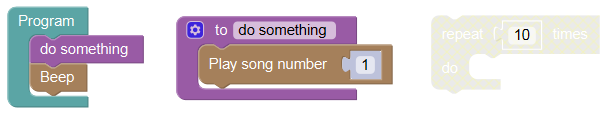
\includegraphics[width=0.95\textwidth]{images/disabled-orphan-block}}
\caption[Blok umiestnený mimo hlavného programu a definície procedúry]{Blok umiestnený mimo hlavného programu a definície procedúry}
\label{obr:disabled-orphan-block}
\end{figure}

\subsection{Základné bloky, logika, cykly, aritmetika}
Definície blokov kategórií \textit{matematická logika}, \textit{cykly} a \textit{matematika} preberáme od autorov knižnice Blockly. Pri definícii generátora vychádzame z existujúceho, produkujúceho kód v jazyku JavaScript. V aplikácii sú prístupné bloky pre podmienku if, konštanty pravdivostných hodnôt a ich porovnanie, blok pre negáciu, číselné konštanty, unárne mínus, aritmetické operácie a blok pre prístup ku generátoru náhodných čísel. Vyššiu abstrakciu pre logické operácie poskytuje napríklad blok \uv{test vlastnosti čísla}, ktorého návratovou hodnotou je pravdivostná hodnota a používateľovi umožňuje testovať paritu, pozitivitu alebo deliteľnosť čísel na základe slovnej definície tejto vlastnosti (obrázok \ref{obr:block-number-property}).

V kategórii cyklov sú k dispozícii bloky pre štandardný cyklus for, while, blok pre príkaz \textit{break} a \textit{continue}. Vyššiu abstrakciu umožňuje špeciálny cyklus, pre ktorý používateľ definuje len počet iterácií. Pri generovaní kódu je potom na jeho mieste vytvorená definícia štandardného cyklu for s lokálnou premennou, ktorou je iterované v postupných inkrementoch od 0 po užívateľom zadané číslo - 1.

\begin{figure}
\centerline{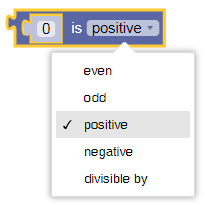
\includegraphics[width=0.35\textwidth]{images/block-number-property}}
\caption[Abstrakcia bloku testujúcého vlastnosť čísla]{Abstrakcia bloku testujúcého vlastnosť čísla}
\label{obr:block-number-property}
\end{figure}

\subsection{Premenné}
Dôležitým komponentom jazyka sú premenné. Blockly je potrebné prispôsobiť pre použitie typových premenných jazyka C, pričom autori podobných aplikácií pristupujú k riešeniu premenných rôzne. V online webovej verzií editora MakeCode (riadenie robota Lego Mindstorms) sú k dispozícii len číselné premenné, textové reťazce a binárne hodnoty môžu byť len konštantou \cite{makeCodeWebEditor}. Na druhej strane, v produkte Otto Blockly je možné vytvoriť premennú typu znak, reťazec, celé číslo, desatinné číslo i binárna hodnota. K dispozícií sú bloky pre inicializáciu, priradenie, i získanie hodnoty premennej. Typy nie sú však vizuálne výraznejšie odlíšené. V editore kódu možno deklarovať premennú binárneho typu a následne iným blokom túto premennú inkrementovať, na čo validátor bloku oznámi chybu. Otázne však je, či je vhodné povoliť vytvorenie neprípustného spojenia. V našej aplikácii vynucujeme určenie typu premennej pri jej vytváraní, bez možnosti dodatočnej zmeny. Povolené typy sú celé číslo (int16\_t), textový reťazec (String) a binárna hodnota (bool). Bloky pre priradenie do premennej a čítanie premennej majú pre jednoznačnosť v rámci typu rovnakú farbu. Správnosť typu je vynucovaná pri každom pokuse o spojenie blokov.

\subsection{Procedúry a funkcie}
Bloky pre vytváranie procedúr a funkcií boli modifikované pre podporu typových premenných. V definícii funkcie je nutné deklarovať typ parametrov a pri volaní je následne vynucovaný. Pre tento účel bola rozšírená ponuka dialógového okna pre úpravu počtu parametrov funkcie (obrázok \label{obr:pocedure-definition}).

Komplikáciou pri práci s procedúrami a funkciami je určenie rozsahu platnosti premenných, ich argumentov. V Blockly je pre vytváranie premenných štandardne určená jedna z položiek menu ponuky prvkov GPJ. Sú v nej zobrazené všetky vytvorené premenné, lokálne i globálne, všetky, čo boli v editore deklarované. Môže tak ľahko dôjsť k zmätočnej situácii, keď deklarujeme rovnomennú premennú iného typu v rámci dvoch procedúr a v menu poskytujúcom prístup k premenným sú naraz dostupné obe. Riešením je vynucovanie typu pre raz definovaný názov premennej. Takto možno všetky používateľom vytvorené premenné vyhlásiť za globálne a predísť nežiadaným situáciám.

Blok pre definíciu funkcie bol modifikovaný doplnením pola pre explicitnú špecifikáciu návratového typu.

\begin{figure}
\centerline{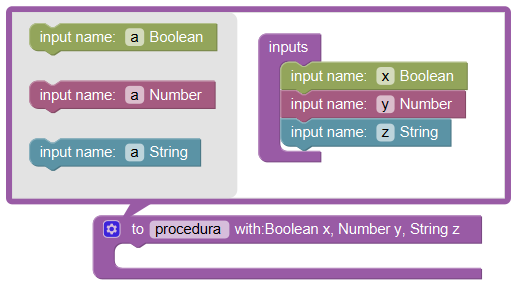
\includegraphics[width=0.75\textwidth]{images/pocedure-definition}}
\caption[Definícia argumentov procedúry]{Definícia argumentov procedúry}
\label{obr:pocedure-definition}
\end{figure}

\subsection{Ovládanie zvukových efektov a mp3 prehrávača}



\subsection{Ovládanie senzorov}

\subsection{Sériová komunikácia prostredníctvom USB}

\subsection{Sériová komunikácia prostredníctvom Bluetooth}


\subsection{Bloky pre prácu s časom}


\subsection{Iné bloky}


\subsection{Generátor kódu}















